% CVIS & J-CVIS latex template
% This template was created by modifying the template from ICCV 2025 (https://www.overleaf.com/latex/templates/iccv2025-author-kit/nwnvrwcqwcsh)


\documentclass[11pt,letterpaper]{article}

%%%%%%%%% PAPER TYPE  - PLEASE UPDATE FOR FINAL VERSION
% \usepackage{cvis}              % To produce the CAMERA-READY version
% \usepackage[review]{cvis}      % To produce the REVIEW version
\usepackage[pagenumbers]{cvis} % To force page numbers, e.g. for an arXiv version

\usepackage{setspace}
\singlespacing  % Put this in preamble or where you want single spacing

% Import additional packages in the preamble file, before hyperref
\input{preamble}

% It is strongly recommended to use hyperref, especially for the review version.
% hyperref with option pagebackref eases the reviewers' job.
% Please disable hyperref *only* if you encounter grave issues, 
% e.g. with the file validation for the camera-ready version.
%
% If you comment hyperref and then uncomment it, you should delete *.aux before re-running LaTeX.
% (Or just hit 'q' on the first LaTeX run, let it finish, and you should be clear).
\definecolor{cvisblue}{rgb}{0.21,0.49,0.74}
\usepackage[pagebackref,breaklinks,colorlinks,allcolors=cvisblue]{hyperref}
%%%%%%%%% PAPER ID  - PLEASE UPDATE
% \def\paperID{*****} % *** Enter the Paper ID here
\def\confName{CVIS}
\def\confYear{2026}

%%%%%%%%% TITLE - PLEASE UPDATE
\title{Season 2026 UWaterloo Robotics Preliminary Design Review}

%%%%%%%%% AUTHORS - PLEASE UPDATE
\author{Yuchen Lin; Saheed Quadri\\
University of Waterloo\\
200 University Ave W, Waterloo\\
{\tt\small y29lin@uwaterloo.ca; s3quadri@uwaterloo.ca}
% For a paper whose authors are all at the same institution,
% omit the following lines up until the closing ``}''.
% Additional authors and addresses can be added with ``\and'',
% just like the second author.
% To save space, use either the email address or home page, not both
}

\begin{document}
\maketitle    
\begin{abstract}
After a successful reveal of our 2025 Rover vehicle platform - Sparky. For the 2026 URC competition season, the UW Robotics team presents Sparky revamped with a handful of upgrades and stress testing results. This year, our team continued to focus on validating the old system benchmarking the performance and implementing a lot of new software patches for system update.
\end{abstract}    
\section{Introduction}
\label{sec:intro}

The University of Waterloo Robotics Team (UWRT) is a dynamic, student-led team of over 50 members from engineering, math, and science programs, including Mechatronics Engineering, Systems Design Engineering, and Computer Science. A multifaceted group with 70\% of members joining to extend diverse backgrounds of highschool robotics enrichment in FIRST, VEX and other forms, UWRT members are inspired by real world applications of robotics with tangible lasting impacts. In the past, the team has participated in the Autonomous Robot Racing competition, mini sumo competition, Intelligent Ground Vehicle competition, and has participated in the University Rover Challenge as our main competition since 2010. UWRT Alumni go on to found industry leading robotics organizations, fostering  team history that ripples through and connects current members to exciting opportunities.

This year, the team adopted a streamlined two-level hierarchy to enhance collaboration. Team Leads oversee high-level rover architecture, system integration, roadmapping, and external communications. Subteam Leads focus on subsystem implementation and onboarding, ensuring that member designs align with the team’s objectives. New members benefit from onboarding training, shadowing opportunities, and personalized mentorship from Subteam Leads. UWRT actively participates in Open House events and community outreach initiatives, inspiring future generations through programs and tours for elementary and middle school students, proudly representing the University of Waterloo and its mission. 

The team operates out of a dedicated design bay in the University of Waterloo’s engineering building, equipped with tools such as 3D printers and soldering stations. Additional support from university facilities, including the machine shop and paint room, enables complex manufacturing. Funding is sourced from university organizations such as WEEF and EngSoc, along with industry sponsors, supporting prototyping, testing, and team operations. A financial statement is detailed in Table 1.

 
\section{Administrative Information}
\label{sec:plan}

\subsection{Team Resources}

The team operates from a dedicated design bay at the University of Waterloo, equipped with mechanical and prototyping. Additional support from university facilities, including the machine shop and paint room, enables complex manufacturing. Funding is sourced from university organizations such as WEEF and EngSoc, along with industry sponsors like Kenesto, QNX, and ProtoSpace Mfg, supporting prototyping, testing, and team operations. A financial statement is detailed in figure \ref{fig:uwrt_balance}. This year, our budget is allocated to three main areas: upgrading specific rover functionality such as wheels for improved grip on rocky terrain, acquiring higher-performance components like high-torque motors, and maintaining spare components for failures during testing.

 \subsection{Project Managment Plan}

Upon release of the URC 2026 requirements, our team break down our rover development cycle into three interconnected phases: functional validation, feature integration, and system-level testing. After PDR submission, all subsystems complete independent functional testing to validate core component performance. Prior to System Acceptance Review, we will develop a minimal viable product demonstrating core system capability across navigation, manipulation, and science tasks. After MVP validation, we will fix stability issues and conducts final system-level testing for competition readiness. The team's project schedule is detailed in the Gantt chart (Figure \ref{fig:uwrt_gantt}), which specifies responsible subteams, task dependencies, and critical dates.Confluence serves as the primary knowledge management system for technical documentation and meeting minutes. 

Integration follows a structured bottom-up approach where subsystems are independently validated before integrated, highlighting modularity in design. System validation occurs through three progressive stages: Software-in-the-Loop testing using Gazebo simulation for algorithm validation, Hardware-in-the-Loop testing with emulated sensors for system behavior performance, and System-Level testing at the Canadesys lunar facility to evaluate rover performance in competition-realistic environments. Testing schedules for each subsystem are labeled into figure\ref{fig:uwrt_gantt}.

\section{Technical Design}
\label{sec:design}

\subsection{System Overview}
\label{subsec:sys_overview}

As illustrated in Figure \ref{fig:rover_sys_arch}, our rover is designed with three primary subsystems: a 35kg drivetrain with 6-wheel rocker bogie suspension powered by a 48V battery, a 6-DoF manipulator with brushless motor-encoder pairs, and a science payload featuring microscope imaging, environmental sensors, and soil sampling capabilities. Most of the rover hardware design is kept from the previous competition cycle, but the goal for this year is to make the design more like a product than a prototype.

\subsection{Season 2026 Updates}
\label{subsec:update}

\subsubsection{Compute Module}
This competition season, our team has welcomed QNX as a key sponsor in our rover development. QNX provides a high-safety, low-latency, real-time operating system running on Raspberry Pi 4B boards with comprehensive support packages. Our key architectural change this year is to replace all low-level STM microcontrollers with two RPi boards serving as I/O expansion modules, enabling preprocessing of sensor data before transmission to Jetson, our main compute module. This preprocessing layer improves system reliability and latency. We continue to use Jetson with ROS2 Humble as our main compute platform, as this solution has proven reliable and effective in previous seasons.

\subsubsection{Power System}

\subsubsection{Communication}

This year instead of implementing both LCM and DDS for comms although the hardware are the same, we are going to unify all the comms.

\subsubsection{Drivetrain}

\subsubsection{Arm}

\subsubsection{Science}

\subsubsection{Ground Station}

\appendix
\section{appendix}
\label{sec:appendix}
\begin{figure}[htp]
    \centering
    \includegraphics[width=0.6\textwidth]{figures/UWRT Team Structure.png}
    \caption{
        UWRT employs a three-level organizational structure. The Team Lead oversees primary communication with university administrators and sponsors, while the Safety Captain ensures compliance with safety standards. The Business Lead manages outreach initiatives and sponsorship agreements. Senior members form an Architecture Decision Committee that reviews and approves all architectural decisions and purchase requests. The third level consists of general team members across mechanical, electrical, firmware, software, and business disciplines who continuously develop and implement new rover features using state-of-the-art algorithms.
    }
    \label{fig:uwrt_team_structure}
\end{figure}

\begin{figure}[htp]
    \centering
    \includegraphics[width=0.8\textwidth]{figures/UWRT PDR Balance Sheet.png}
    \caption{
        UWRT Season 2026 Budget: income (left) and expenses by project (right).
    }
    \label{fig:uwrt_balance}
\end{figure}

% add Mechanical; add testing and integration with detail; add electrical tasks.
% add better caption
\begin{figure}[htp]
    \centering
    \includegraphics[width=0.8\textwidth]{figures/S26 UWRT Gantt Chart.png}
    \caption{
        The Gantt chart illustrates the UWRT S26 project timeline and is organized into two sections. The top section displays key project deadlines, color-coded as follows: red indicates URC competition deadlines, orange marks system functionality milestones, and yellow represents project completion deadlines. The bottom section presents the detailed task timeline for each subteam—Mechanical, Electrical, Firmware, Software, Integration, Testing, and specialized subsystems (Drivetrain, Arm, Science, and Communications)—with color-coded task tracking. The team has structured the project around three major milestones. First, the team focuses on validating the functionality of all primary components, including both commercial off-the-shelf and custom-designed parts. Following PDR document submission, the team will lock in the system architecture for the season. The second milestone targets the system's minimal viable product (MVP). Finally, the team will conduct fine-tuning and stress testing to optimize system performance for the University Rover Challenge competition.
    }
    \label{fig:uwrt_gantt}
\end{figure}

% Where is the Science Module and Ground Station
\begin{figure}[htp]
    \centering
    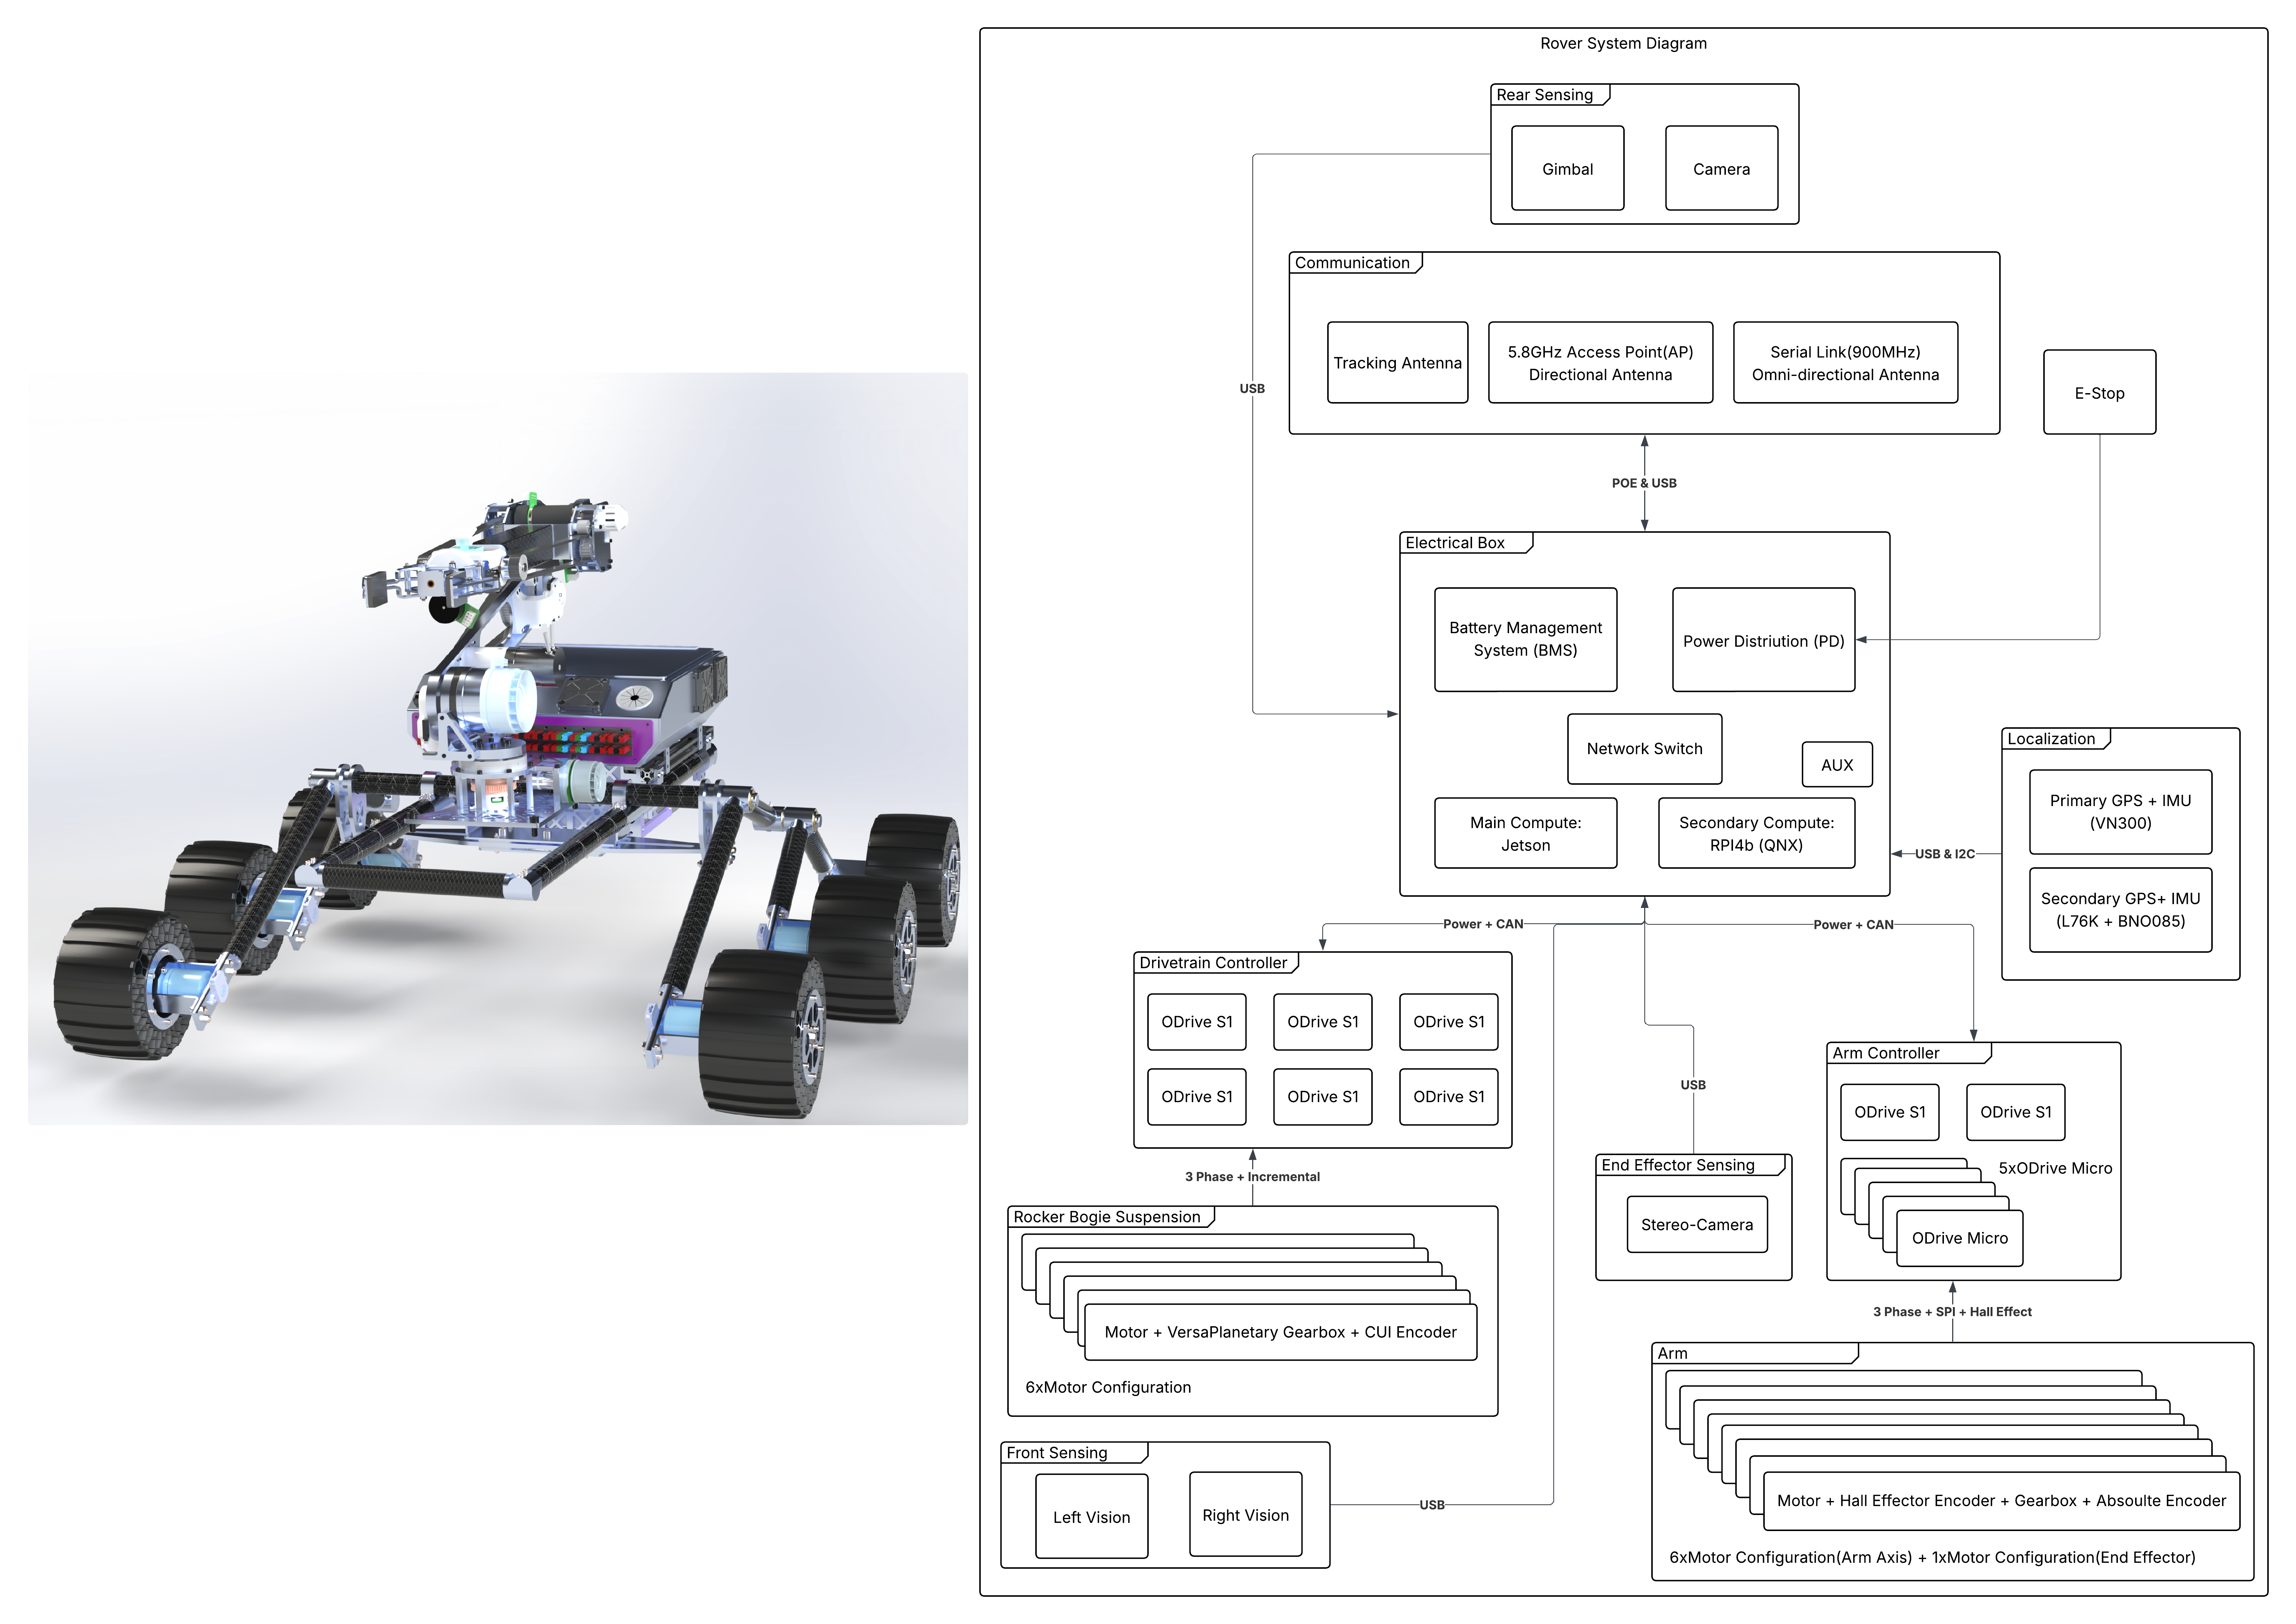
\includegraphics[width=0.8\textwidth]{figures/Rover System Diagram.png}
    \caption{
        This figure shows the main system diagram for the whole rover system. 
        The center is the Electrical Box containing all the main electronics. 
        BMS is for cell balancing. 
        PD is for over-voltage protection, over-current protection, and state of charge monitoring. 
        Jetson is our main controller solving all the kinematics. 
        Raspberry Pi 4B loaded with QNX serves as an IO expansion board and low-level controller. 
        Communication Module transmits UDP packets and communicates with the ground station. 
        The Rear Sensing Module serves as an overview camera for livestreaming the rover status to the ground station. 
        E-Stop performs the critical safety functionality and cuts the high power rail under emergency. 
        Localization has a dual GPS + IMU configuration providing high accuracy location results after sensor fusion. 
        Front Sensing uses two cameras to perform obstacle avoidance and path planning. 
        Drivetrain and Arm systems are described in their own architecture diagrams.
    }
    \label{fig:rover_sys_arch}
\end{figure}


\end{document}
